% Created 2021-03-17 Wed 20:59
% Intended LaTeX compiler: pdflatex

\documentclass[english]{article}
\usepackage[T1, T2A]{fontenc}
\usepackage[lutf8]{luainputenc}
\usepackage[english, russian]{babel}
\usepackage{minted}
\usepackage{graphicx}
\usepackage{longtable}
\usepackage{hyperref}
\usepackage{xcolor}
\usepackage{natbib}
\usepackage{amssymb}
\usepackage{stmaryrd}
\usepackage{amsmath}
\usepackage{caption}
\usepackage{mathtools}
\usepackage{amsthm}
\usepackage{tikz}
\usepackage{grffile}
\usepackage{extarrows}
\usepackage{wrapfig}
\usepackage{rotating}
\usepackage{placeins}
\usepackage[normalem]{ulem}
\usepackage{amsmath}
\usepackage{textcomp}
\usepackage{capt-of}

\usepackage{geometry}
\geometry{a4paper,left=2.5cm,top=2cm,right=2.5cm,bottom=2cm,marginparsep=7pt, marginparwidth=.6in}

 \usepackage{hyperref}
 \hypersetup{
     colorlinks=true,
     linkcolor=blue,
     filecolor=orange,
     citecolor=black,      
     urlcolor=cyan,
     }

\usetikzlibrary{decorations.markings}
\usetikzlibrary{cd}
\usetikzlibrary{patterns}
\usetikzlibrary{automata, arrows}

\newcommand\addtag{\refstepcounter{equation}\tag{\theequation}}
\newcommand{\eqrefoffset}[1]{\addtocounter{equation}{-#1}(\arabic{equation}\addtocounter{equation}{#1})}


\newcommand{\R}{\mathbb{R}}
\renewcommand{\C}{\mathbb{C}}
\newcommand{\N}{\mathbb{N}}
\newcommand{\rank}{\text{rank}}
\newcommand{\const}{\text{const}}
\newcommand{\grad}{\text{grad}}

\theoremstyle{plain}
\newtheorem{axiom}{Аксиома}
\newtheorem{lemma}{Лемма}
\newtheorem{manuallemmainner}{Лемма}
\newenvironment{manuallemma}[1]{%
  \renewcommand\themanuallemmainner{#1}%
  \manuallemmainner
}{\endmanuallemmainner}

\theoremstyle{remark}
\newtheorem*{remark}{Примечание}
\newtheorem*{solution}{Решение}
\newtheorem{corollary}{Следствие}[theorem]
\newtheorem*{examp}{Пример}
\newtheorem*{observation}{Наблюдение}

\theoremstyle{definition}
\newtheorem{task}{Задача}
\newtheorem{theorem}{Теорема}[section]
\newtheorem*{definition}{Определение}
\newtheorem*{symb}{Обозначение}
\newtheorem{manualtheoreminner}{Теорема}
\newenvironment{manualtheorem}[1]{%
  \renewcommand\themanualtheoreminner{#1}%
  \manualtheoreminner
}{\endmanualtheoreminner}
\captionsetup{justification=centering,margin=2cm}
\newenvironment{colored}[1]{\color{#1}}{}

\tikzset{->-/.style={decoration={
  markings,
  mark=at position .5 with {\arrow{>}}},postaction={decorate}}}
\makeatletter
\newcommand*{\relrelbarsep}{.386ex}
\newcommand*{\relrelbar}{%
  \mathrel{%
    \mathpalette\@relrelbar\relrelbarsep
  }%
}
\newcommand*{\@relrelbar}[2]{%
  \raise#2\hbox to 0pt{$\m@th#1\relbar$\hss}%
  \lower#2\hbox{$\m@th#1\relbar$}%
}
\providecommand*{\rightrightarrowsfill@}{%
  \arrowfill@\relrelbar\relrelbar\rightrightarrows
}
\providecommand*{\leftleftarrowsfill@}{%
  \arrowfill@\leftleftarrows\relrelbar\relrelbar
}
\providecommand*{\xrightrightarrows}[2][]{%
  \ext@arrow 0359\rightrightarrowsfill@{#1}{#2}%
}
\providecommand*{\xleftleftarrows}[2][]{%
  \ext@arrow 3095\leftleftarrowsfill@{#1}{#2}%
}
\makeatother
\author{Ilya Yaroshevskiy}
\date{\today}
\title{Практика 4}
\hypersetup{
 pdfauthor={Ilya Yaroshevskiy},
 pdftitle={Практика 4},
 pdfkeywords={},
 pdfsubject={},
 pdfcreator={Emacs 28.0.50 (Org mode )}, 
 pdflang={English}}
\begin{document}

\maketitle
\tableofcontents


\section{Практика 4}
\label{sec:org51b3048}
\begin{itemize}
\item \(x = ar \cos^\alpha\varphi\)
\item \(y = br \sin^\alpha\varphi\)
\end{itemize}
\[ J = \alpha a b r \cos^{\alpha - 1}\varphi\sin^{\alpha - 1}\varphi \addtag\label{4_jord}\]
\[ \frac{y}{x} = \const \cdot \tg^\alpha \varphi \]
\begin{task}
\[ \frac{x^3}{a^3} + \frac{y^3}{b^3} = \frac{x^2}{h^2} + \frac{y^2}{k^2}\quad x = 0,y=0 \]
\end{task}
\begin{solution}
\[ \alpha = \frac{2}{3}\ r = \frac{a^2}{h^2}\cos^{\frac{4}{3}}\varphi + \frac{b^2}{k^2}\sin^{\frac{4}{3}}\varphi \]
Из \ref{4_jord} \(\alpha = \frac{2}{3}\)
\[ \lambda{\Omega} = \iint_\Omega 1 dx dy = \int^{\frac{\pi}{2}}_0 du \int^{r(u)}_0 \frac{2}{3}abr\cos^{\alpha - 1}\varphi\sin^{\alpha - 1}\varphi dr = \]
\[ = \frac{1}{3}ab\int^{\frac{\pi}{2}}_0\cos^{\alpha - 1}\varphi\sin^{\alpha - 1}\varphi\left(\frac{a^2}{h^2}\cos^\frac{4}{3}\varphi + \frac{b^2}{k^2}\sin^\frac{4}{3}\varphi\right)^2d\varphi = \text{I} + \text{II} + \text{III}\]
\[ \text{I} = \int_0^\frac{\pi}{2} \frac{a^4}{h^4}\cos^\frac{7}{3}\varphi\sin^{-\frac{1}{3}}\varphi d\varphi = \left|\substack{t = \sin^2\varphi \\ d\varphi\right. = \frac{1}{2t^\frac{1}{2}(1 - t)^\frac{1}{2}}} = \frac{a^4}{b^4} \int_0^1 (1 - t)^{\frac{7}{6} - \frac{1}{2}}t^{-\frac{1}{6} - \frac{1}{2}} = \frac{a^4}{2b^4}B(\frac{5}{3}, \frac{1}{3})\]
\end{solution}
\begin{task}
\[ (x^3 + y^3)^2 = x^2 + y^2 \]
, \(x \ge 0, y \ge 0\) \(\to\) полярные координаты
\end{task}
\begin{solution}
\[ r^4(\cos^3\varphi + \sin^3\varphi) = 1 \]
\[ \lambda(\Omega) = \int^\frac{\pi}{2}_0 d\varphi \int^{r(\varphi)}_0 \underset{\substack{\uparrow \\ \text{Якобиан}}}{r} dr = \frac{1}{2}\int^\frac{\pi}{2}_0 \frac{d\varphi}{\cos^3\varphi + \sin^3\varphi} = \frac{1}{2} \int_0^{ + \infty} \frac{\sqrt{t^2 + 1}}{t^3 + 1}dt \]
\[ \int \frac{d\varphi}{(\cos \varphi + \sin\varphi)(1 - \cos\varphi\sin\varphi)} \]
\[ \int \frac{dt}{\left(\frac{2t^2}{1 + t^2}\right)^3 + \left(\frac{2t}{1 + t^2}\right)^3} \cdot \frac{2}{1 + t^2} \]
\end{solution}
\begin{task}
\[ \left(\frac{x}{a}\right)^\frac{2}{3} + \left(\frac{y}{b}\right)^\frac{2}{3} = 1 \]
\[ \left(\frac{x}{a}\right)^\frac{2}{3} + \left(\frac{y}{b}\right)^\frac{2}{3} = 4 \]
, \(\frac{x}{a} = \frac{y}{b},\ 8\frac{x}{a} = \frac{y}{b}\)
\end{task}
\begin{solution}
\[ \begin{array}{l} x = ar \cos \varphi^3 \\ y = b r \sin^3 \varphi \end{array} \]
\begin{itemize}
\item \(r = 1, r = 8\)
\item \(\varphi = 1, \varphi = \arctg 2\)
\end{itemize}
\[ \lambda(\Omega) = \int^8_1 dr \int ^{\arctg 2}_1 3 ab r \cos^2\varphi \sin^2 \varphi d\varphi = \frac{3}{2} ab r^2 \bigg^8_1\cdot \underbrace{\int^{\arctg 2}_1 \sin^2 2\varphi d\varphi}_{\displaystyle\frac{1 - \cos 4\varphi}{2}}\]
\end{solution}
\begin{task}
\[ xy = a^2 \]
\[ x + y = \frac{5}{2} \]
\end{task}
\begin{solution}
\-
\begin{center}
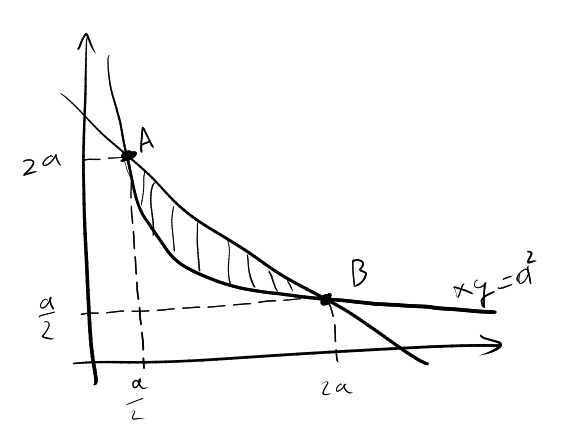
\includegraphics[scale=0.3]{4_1.png}
\end{center}
\[ \int^{2a}_{\frac{a}{2}}\int^{\frac{5}{2}a - x}_{\frac{a^2}{x}} dy = q^2 \frac{15}{8} - 2q^2 \ln 2 \]
\[  = \int^{2a}_{\frac{a}{2}} \frac{5}{2} a - x - \frac{a^2}{x} dx = \frac{5}{2} a \cdot \frac{3}{2} a - \frac{x^2}{2}\bigg|^{2a}_{\frac{a}{2}} - a^2 \ln x \bigg|^{2a}_{\frac{a}{2}}\]
\end{solution}
\begin{task}
\[ xy = a^2 \]
\[ xy = 2a^2 \]
\[ y = x \]
\[ y = 2x \]
, \(x, y > 0\)
\end{task}
\begin{solution}
\-
\begin{center}
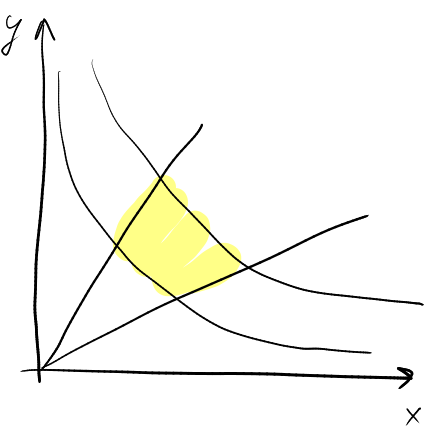
\includegraphics[scale=0.3]{4_2.png}
\end{center}
\[ u = xy,\ v = \frac{y}{x} \]
\[ x = \sqrt{\frac{u}{v}} \]
\[ y = \sqrt{uv} \]
\[ J = \begin{vmatrix}\frac{1}{2\sqrt{uv}} & -\frac{1}{2}\frac{\sqrt{u}}{\sqrt{v}} \\ \frac{1}{2} \frac{\sqrt{v}}{\sqrt{u}} & \frac{1}{2}\frac{\sqrt{u}}{\sqrt{v}} \end{vmatrix} = \frac{1}{2v} \]
\[ \lambda(\Omega) = \int^{2a^2}_{a^2}du\int^2_1 \frac{1}{2v} dv = a^2 \int^2_1 \frac{1}{2v}dv = \frac{a^2}{2}\ln 2 \]
\end{solution}
\begin{task}
\[ V = \int^1_0 dx \int ^{1 - x}_0 x^2 + y^2 dy \]
Определим что эта за фигура в плоскости \(xOy\)
\begin{center}
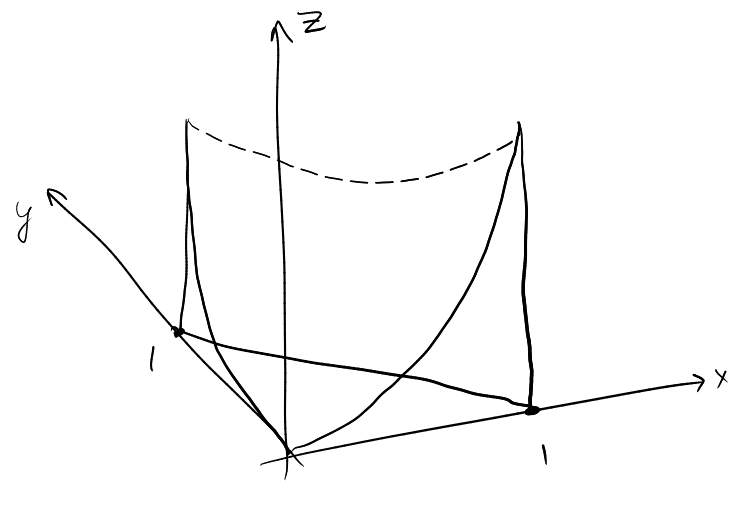
\includegraphics[scale=0.5]{4_3.png}
\end{center}
\end{task}
\begin{task}
\[ \left[\begin{array}{l} z = 1 + x + y \\ z = 0\end{array}\right. \]
\[ \left[\begin{array}{l} x + y = 1 \\ x = 0 \\ y = 0 \end{array}\right. \]
Цилинрическая форма
\begin{center}
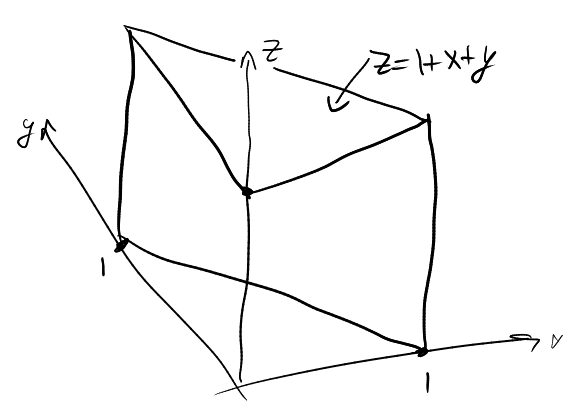
\includegraphics[scale=0.5]{4_5.png}
\end{center}
\end{task}
\begin{solution}
\[ \lambda(\Omega) =\int^1_0 dx \int^{1 - x}_0 1 + x + y dy = \int^1_0(1 + x)(1 - x) + \frac{y^2}{2}\bigg^{1 - x}_0 dx \]
\end{solution}

\begin{task}
\[ \left[\begin{array}{l} z^2 = xy \\ x^2 + y^2 = a^2 \end{array}\right. \]
\begin{center}
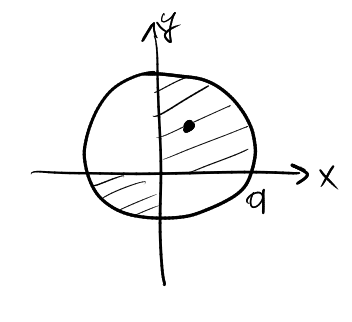
\includegraphics[scale=0.5]{4_4.png}
\end{center}
\end{task}
\begin{solution}
\[ \lambda(\Omega) = 4 \iint \sqrt{xy} dx dy = \int^{\frac{\pi}{2}}_0 d\varphi \int^a_0 r^2 \sqrt{\cos\varphi\sin\varphi} dr = \frac{a^3}{3} \int^{\frac{\pi}{2}}_0 \cos^{\frac{1}{2}}\varphi \sin^{\frac{1}{2}}\varphi d\varphi\]
\end{solution}
\begin{task}
\[ \frac{x^2}{a^2} + \frac{y^2}{b^2} + \frac{z^2}{c^2} = 1 \]
\[ \frac{x^2}{a^2} + \frac{y^2}{b^2} = \frac{z^2}{c^2} \]
\begin{center}
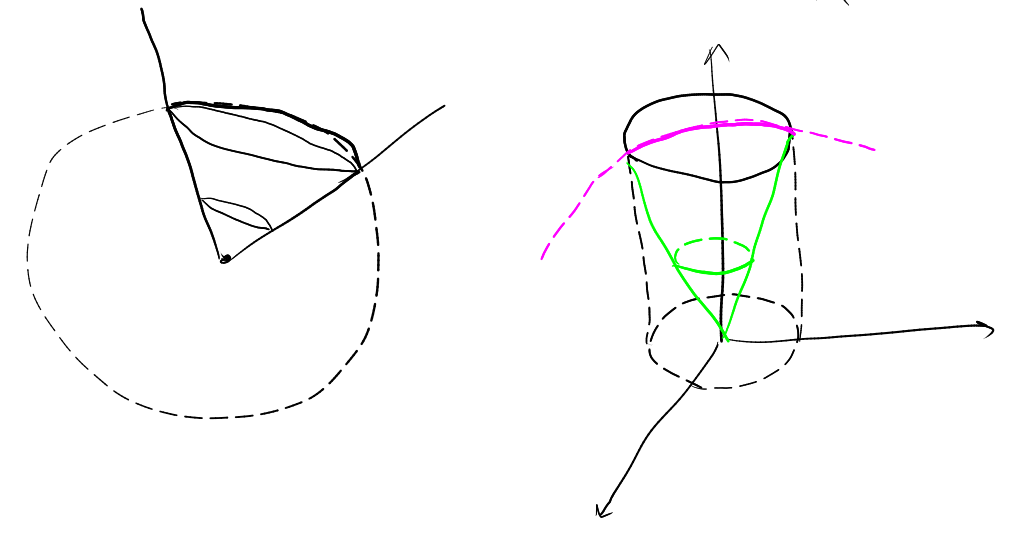
\includegraphics[scale=0.4]{4_6.png}
\end{center}
\end{task}
\begin{solution}
\[ V = \iint z_2 (x, y) - z_1(x, y) \addtag\label{4_9_1}\]
\[\frac{2z^2}{c^2} = 1\]
\[ z = \frac{c}{\sqrt{2}} \]
\[ \frac{x^2}{a^2} + \frac{y^2}{b^2} = \frac{1}{2} \]
\[ \ref{4_9_1} = \left|\begin{array}{l}x = ar\cos \varphi \\ y = br\sin\vaprhi\end{array}\right. = \int^{2\pi}_0 d\varphi \int^{\frac{1}{\sqrt{2}}}_0 abr(-c^2\cdot r^2 + c^2(1 - r^2)) = 2\pi \int^{\frac{1}{\sqrt{2}}}_0\]
\end{solution}

\begin{task}
\[ z^2 = xy \]
\[ x + y = a \]
\[ x + y = b \]
\begin{center}
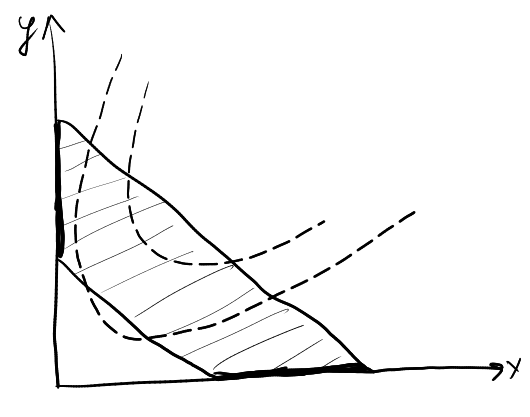
\includegraphics[scale=0.5]{4_7.png}
\end{center}
\end{task}
\begin{solution}
\[ 2 \int^b_a dx \int^{a - x}_0 \sqrt{xy} dy + \int^a_0 dx \int^{b - x}_{a - x}\sqrt{xy}dy \]
\end{solution}
\end{document}
